\documentclass[11pt, a4paper]{article}

\usepackage{style}

\author{Vladislav Mlejnecký}

\title{%
  Číslicové zpracování signálů\\
  \large Úloha číslo 8.\\
  Aplikace filtrů na akustický signál}

\begin{document}

    \maketitle

    \section{Zadání}
    
        Cílem cvičení je ukázat, jak zvolený filtr ovlivní signál. 
        Filtr budeme aplikovat na hudební signál v kvalitě CD audio.
    
        \begin{enumerate}
            \item        
            Na signál aplikujte pásmovou propust 300 až 3400 Hz (telefon) a přehrajte, dále nakreslete
            spektrogram (závislost krátkodobého spektra signálu na čase) původního a filtrovaného
            signálu.
            \item        
            Proveďte decimaci signálu 1:5, podobně jako ve cvičení 3.
            Dále proveďte tutéž decimaci u filtrovaného signálu filtrem, navrženým tak, aby
            nedocházelo k aliasingu. Výsledky přehrajte a nakreslete do jednoho obrázku spektrum
            původního signálu, a spektra obou decimovaných signálů (s aliasingem a bez něj).
            \item        
            Načtěte signál ukázky. Přidejte signál o kmitočtu 2200Hz. Navrhněte úzkopásmovou zádrž
            tak, aby se ze signálu přidaný tón (pískání) odfiltroval. Ve všech třech případech ukázku
            přehrajte a nakreslete spektrogram. Aplikujte filtr naprogramovaný podle realizační
            struktury, nikoliv funkce Matlabu filter.
        \end{enumerate}
        
    \section{Výsledné grafy}
        
        \subsection{Telefonní pásmová propust}
        
            \begin{figure}[H]
                \centering
                \begin{minipage}{.5\textwidth}
                    \centering
                    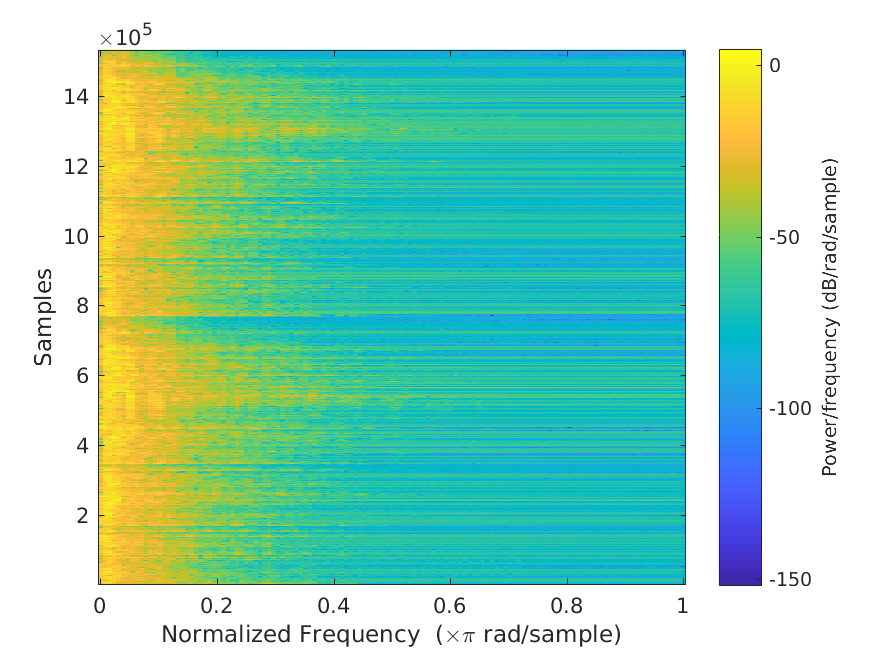
\includegraphics[width=.9\textwidth]{matlab/1_orig.png}
                    \caption{Původní signál}
                    \label{fig:1}
                \end{minipage}%
                \begin{minipage}{.5\textwidth}
                    \centering
                    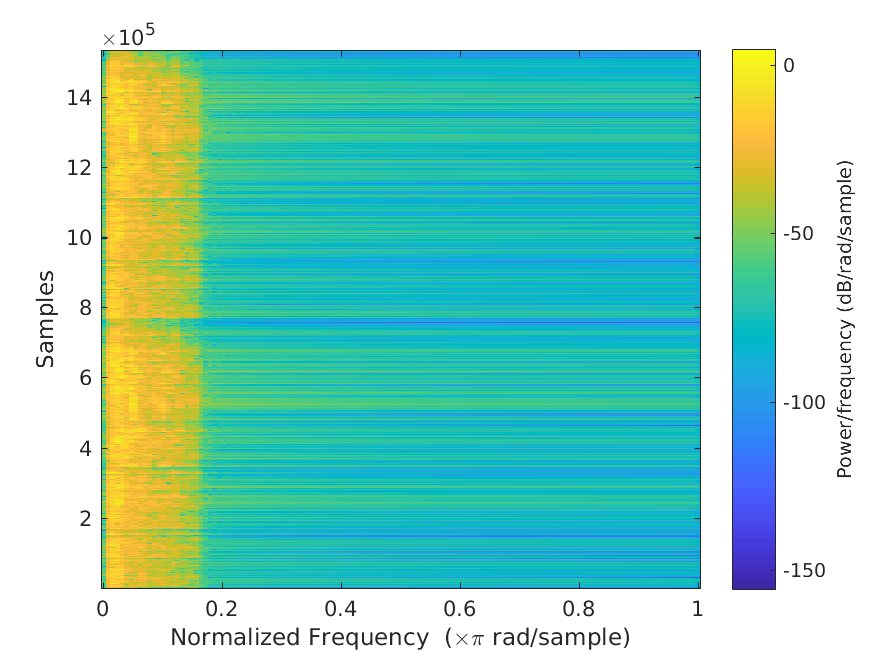
\includegraphics[width=.9\textwidth]{matlab/1_filter.png}
                    \caption{Filtrovaný signál}
                    \label{fig:2}
                \end{minipage}
            \end{figure}
        
        \subsection{Decimace}
        
            \begin{figure}[H]
                \centering
                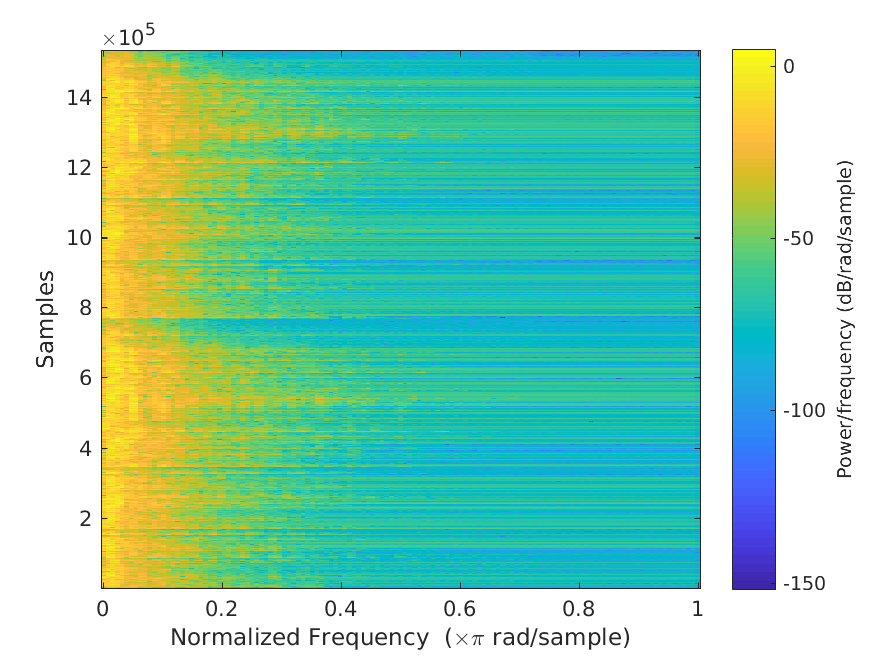
\includegraphics[width=.45\textwidth]{matlab/2_orig.png}
                \caption{Původní spektrum skladby}
                \label{fig:3}
            \end{figure}
        
            \begin{figure}[H]
                \centering
                \begin{minipage}{.5\textwidth}
                    \centering
                    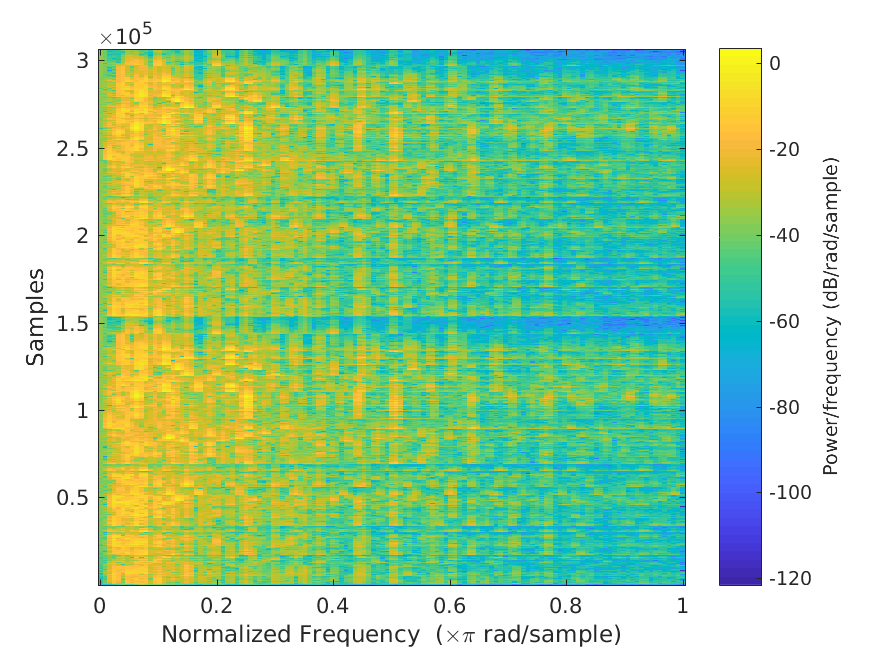
\includegraphics[width=.9\textwidth]{matlab/2_nofilter.png}
                    \caption{Decimace bez filtru}
                    \label{fig:4}
                \end{minipage}%
                \begin{minipage}{.5\textwidth}
                    \centering
                    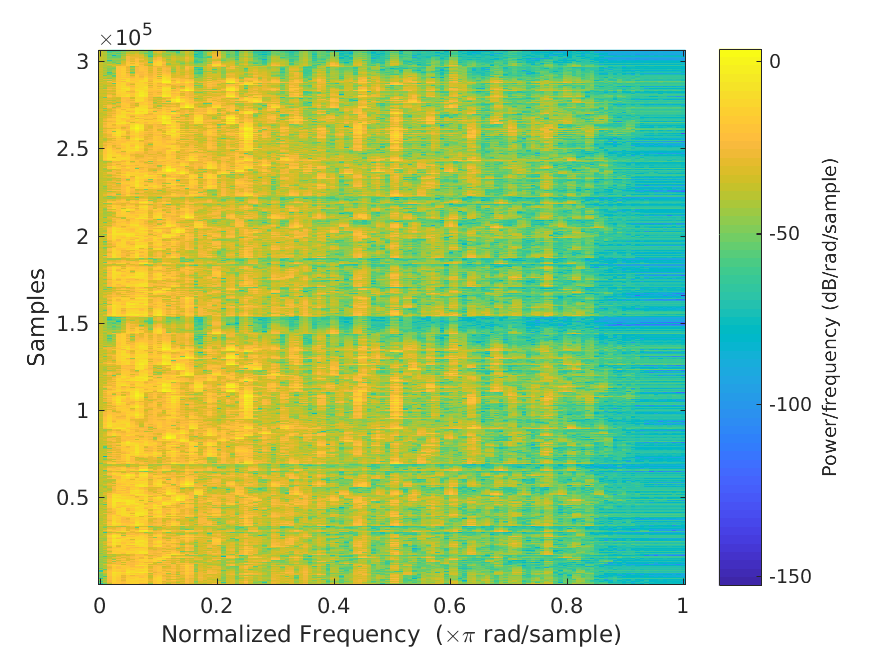
\includegraphics[width=.9\textwidth]{matlab/2_filter.png}
                    \caption{Decimace s filtrem}
                    \label{fig:5}
                \end{minipage}
            \end{figure}
        
        \subsection{Přidaný tón}
        
            \begin{figure}[H]
                \centering
                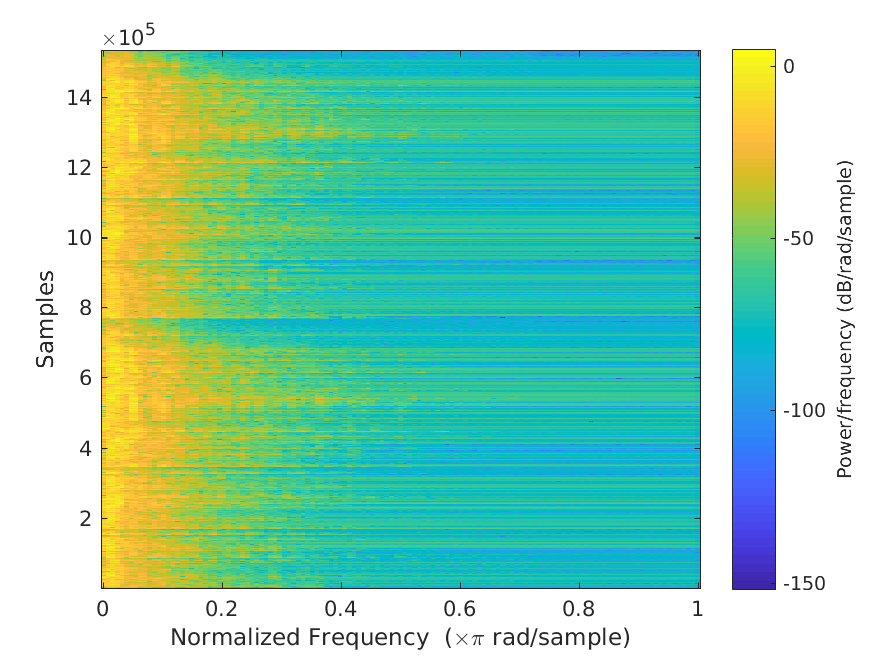
\includegraphics[width=.45\textwidth]{matlab/3_orig.png}
                \caption{Původní spektrum skladby}
                \label{fig:6}
            \end{figure}
        
            \begin{figure}[H]
                \centering
                \begin{minipage}{.5\textwidth}
                    \centering
                    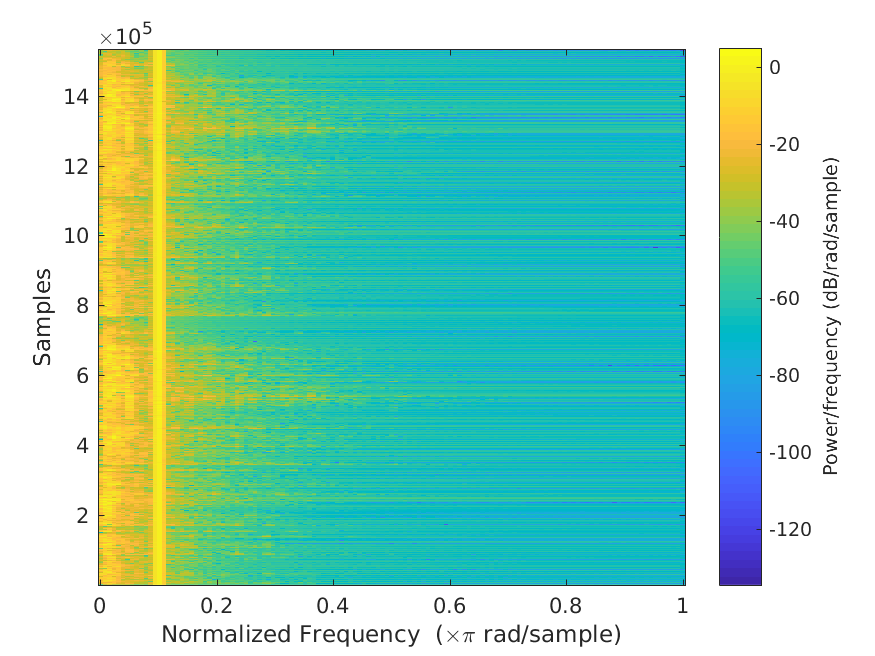
\includegraphics[width=.9\textwidth]{matlab/3_noise.png}
                    \caption{Přidaný signál}
                    \label{fig:7}
                \end{minipage}%
                \begin{minipage}{.5\textwidth}
                    \centering
                    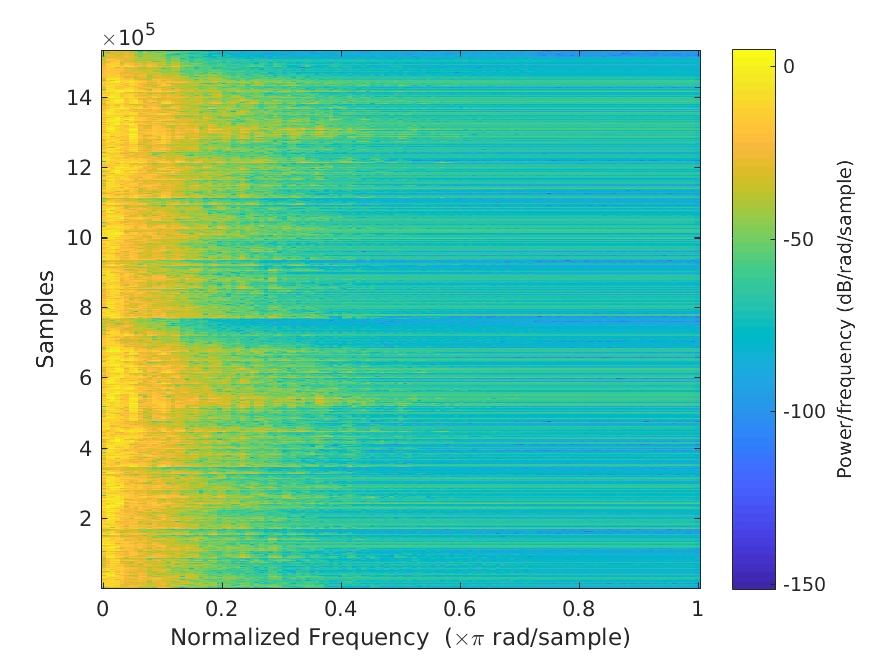
\includegraphics[width=.9\textwidth]{matlab/3_filter.png}
                    \caption{Skladba po filtraci}
                    \label{fig:8}
                \end{minipage}
            \end{figure}
        
    \section{Výpis zdrojového kódu}

\begin{lstlisting}[language=matlab, frame=single] 
mute = 1;
ukol1('Ukaz2Polon.wav', mute);
ukol2('Ukaz2Polon.wav', mute);
ukol3('Ukaz2Polon.wav', mute);

function ukol1(FileName, mute)
    %read file
    [ukazka_orig, Fs_orig] = audioread(FileName);
    
    %play original
    play_muteable(ukazka_orig, Fs_orig, mute);
    
    %filter it
    Fstop = [300 3400];
    [b, a] = cheby1(6, 3, (2/Fs_orig) .* Fstop, 'bandpass');
    y1 = filter(b, a, ukazka_orig);

    %play filtered
    play_muteable(y1, Fs_orig, mute);
    
    %make spectrograms
    make_specgram(ukazka_orig, '1_orig');
    make_specgram(y1, '1_filter');
    
    clear b a y1 ukazka_orig Fs_orig Fstop;
end

function ukol2(FileName, mute)
    [ukazka_orig, Fs_orig] = audioread(FileName);
    
    %decimate without lowpass
    y1 = my_decimate(ukazka_orig, 5);
    y1_fs = Fs_orig / 5;
    
    %decimate with lowpass
    y2 = decimate(ukazka_orig, 5);
    y2_fs = Fs_orig /5;
    
    %play everything
    play_muteable(ukazka_orig, Fs_orig, mute);
    play_muteable(y1, y1_fs, mute);
    play_muteable(y2, y2_fs, mute);
    
    %draw everything
    make_specgram(ukazka_orig, '2_orig');
    make_specgram(y1, '2_nofilter');
    make_specgram(y2, '2_filter');
    
    clear y1 y2 y1_fs y2_fs ukazka_orig Fs_orig;
end

function ukol3(FileName, mute)

    %read file
    [y_orig, Fs_orig] = audioread(FileName);

    %add noise
    t = (0:length(y_orig)-1)/Fs_orig;
    t = transpose(t);
    y_noise = y_orig + 0.25 .* sin(2 * pi * 2200 * t);
    
    %filter noise
    Fstop = [2190 2210];
    [b, a] = butter(1, (2/Fs_orig) .* Fstop, 'stop');
    y_filter = filter(b, a, y_noise);
    
    %draw specgrams
    make_specgram(y_orig, '3_orig');
    make_specgram(y_noise, '3_noise');
    make_specgram(y_filter, '3_filter');
    
    %play everything
    play_muteable(y_orig, Fs_orig, mute);
    play_muteable(y_noise, Fs_orig, mute);
    play_muteable(y_filter, Fs_orig, mute);
    
    clear y_orig y_noise y_filter Fs_orig t;
end

function audio = my_decimate(x, factor)
    n = 1:factor:length(x);
    audio = x(n);
end

function play_muteable(vector,Fs, mute)
    if mute == 0
        obj = audioplayer(vector,Fs);
        playblocking(obj);
        clear obj;
    end
end

function make_specgram(vector, FileName)
    h = figure();
    spectrogram(vector, 256, 10, 256);
    saveas(h, [FileName '.png']);
    close(h);
    clear h;
end
\end{lstlisting}

\end{document}
